\documentclass[pdftex,12pt,letter]{article}
\usepackage[margin=0.75in]{geometry}
\usepackage{verbatim}
\usepackage{graphicx}
\usepackage{xspace}
\usepackage{cite}
\usepackage{url}
\usepackage[pdftex,pdfpagelabels,bookmarks,hyperindex,hyperfigures]{hyperref}

\newcommand{\pd}{protoDUNE\xspace}
%\newcommand{\pdsp}{pD/SP\xspace}
\newcommand{\xrd}{XRootD\xspace}
\newcommand{\expname}{\textit{NP04}\xspace}

\title{A Design of the Prompt Processing System for the Single-Phase \pd experiment (\expname)}
\date{\today}
\author{M.\,Potekhin and B.\,Viren}


\begin{document}
\maketitle

\begin{abstract}
\noindent  This note describes design parameters of
the Prompt Processing system in the Single-Phase \pd
(CERN experiment \expname), and one particular design option for such system
based on prioritized queue. We start with a brief summary of the data characteristics and data handling patterns
as documented in DocDB\,1086 \cite{docdb1086}, DocDB\,1212 \cite{docdb1212} and present
the basic requirements as per  DocDB 1811 \cite{docdb1811}. A design is proposed which satisfies 
these requirements.
\end{abstract}

%%%%%%%%%%%%%%%%%%%%%%%%%%%%%%%%%%%%%%%%%%%%%%%%%%%%%

\section{Overview}
\subsection{Data Scenarios and Data Handling}
\label{sec:rawdata}
Quantitative information about scenarios for data taking in \pd is collected and maintained in \cite{docdb1086}. The following parameters
are assumed at the time of writing: the raw data rate will 1.4\,GB/s after lossless compression, and to size up
the system and account for contingencies rates up to 3\,GB/s are under consideration.

Outline of the design of the raw data handling system is documented in  \cite{docdb1212} and other prior \pd documentation.
According to it, the data is transmitted from the online buffer to the CERN EOS via a 20 Gbps full-duplex network connection.
The EOS system serves as the hub and staging area for the \pd raw data from which
it gets committed to the tape archive at CERN and also transmitted to FNAL and potentially
other US and international locations. All or most links in the data transmission chain will be based on F-FTS.

\subsection{Goals}
\label{sec:outline}
According to \cite{docdb1811}  prompt processing needs to occur on the scale
of tens of minutes (or better) from the time the data was taken. Its purpose is to
provide a more in-depth data QA and assessment of the detector's health and operating conditions
than is afforded by most basic histogramming e.g.~of the ADC counts in individual channels. Most calculations
done as a part of prompt processing will result in some sort of a ``visual product'', for example a histogram,
plot, event display or a summary table in order to provide optimal accessibility to the experiment
operators.


\subsection{Scope of the Prompt Processing}
This is a compressed summary of information presented in \cite{docdb1811}.
For more detailed explanation please see the source.

\subsubsection{Data Processing}
\label{sec:categories}
The categories are as follows:

\begin{description}

\item[DAQ] A summary of DAQ-level data (with no decompression) such as summaries of data
 rates  or summaries of any metadata, status codes the provided by the DAQ etc.
This processing is a candidate for running directly within artDAQ
monitor processes instead of prompt-processing and is included here
for completeness.

\item[ADC] A summary of ADC-level data e.g. mean/RMS (requires data decompression).


\item[FFT] A summary of the ADC-level data in frequency space. It requires running a discrete Fourier
transform (FFT) on channel waveforms. This largely  provides measures of noise and its
evolution.

\item[Sig] A summary of the data \textit{after signal processing}.
The processing is in  both time domain and in frequency domain (so uses the output of FFT).
It includes items such as
\begin{itemize}
\item ``stuck code'' mitigation
\item coherent noise removal
\item noise subtraction and filtering
\item deconvolution of the response function
\item calculation of signal correlations for diagnostic purposes
\end{itemize}

\item[Reco] Results from running some type of reconstruction (perhaps simplified).
It may, for  example, provide a coarse count of straight muon track candidates.

\end{description}


\noindent It is possible that \textbf{ADC} and \textbf{FFT} stages will be implemented as a single processing
block since \textbf{FFT} will require uncompressed data in any case. Likewise, some other stages in the processing
chain and visualization may be conflated in case writing out intermediate (transient) data creates an I/O bottleneck,
while still preserving modularity to the largest extent possible. Such design decisions will be made at a later time.

Note that the categories listed above can be thought of as stages of processing (for the most part), where
the output of a stage serves as input to the next one. This can be conceptualized as a DAG (see \ref{sec:dag}).

\subsubsection{Sampling (pre-scaling) the Data in the Prompt Processing Chain}
\label{sec:downsampling}
The categories of processing as outlined above may have drastically different resource requirements.
%i.e. the ability to select a fractional sample of the data stream as is progresses through the chain, at every stage.
For example, if 100 cores are allocated to FFT calculation this may be done for approximately 10\% of the events
in streaming mode. Then, depending on the type of deconvolution being employed (1D vs 2D) this step
may require an order of magnitude more CPU to complete. To stay within reasonable footprint,
it may be necessary to put only a fraction of the output of the FFT stage through deconvolution stage
(note that the FFT output is valuable in and by itself since it allows to ascertain noise conditions in individual channels
on a continuous basis). Event reconstruction will in turn require even more CPU
and so it may also be necessary to scale down the number of
events at this stage (while still aiming for quick turnaround). So effectively we are considering ``downsampling''
or ``prescaling'' 
of data as it progresses in the prompt processing chain, whereby a certain predetermined fraction of the data
produced in a prompt processing stage is selected for processing in the next stage.
This can be achieved by two methods or some combination thereof:
\begin{itemize}
\item Selecting a fraction of files produced by the previous stage
\item Reading only a fraction of events from a given input file
\end{itemize}

\noindent Parameters governing this fractional data selection must be dynamically configurable.


\subsubsection{Visualization}
\label{sec:viz_intro}

The \textit{Visualization} category of processing
 may take data output from any of the above listed stages in
order to efficiently present it to the end-user. 
% This stage will need to
%have a sampling fraction  based on both the processing requirements
%(e.g. processing time) and based on how fast a human can absorb and understand
%the information as it undergoes updates.
It may include items such as:

\begin{itemize}

\item Histograms of statistical quantities and strip charts showing their history.

\item Various statistics dynamically updated over some some fixed time window.

\item 2D displays of underlying values such as spectrograms of the \textbf{FFT}
  output (vs wire), or time vs wire using output from \textbf{ADC} and \textbf{Sig}.

\end{itemize}

\subsubsection{Other Applications of the Data Processing Components}
Results of the intermediate stages of Data Processing may need to be preserved, for
example the data in graphic form for audit/run documentation purposes.
Also, there could be a potential for large processing efficiency
gains to be made if the entire data can be run through the \textit{Sig} processing followed by ZS.
Certain portion of log files produced during prompt processing may contain information useful
for future reference and debugging, so provisions will be made to capture these data.


\section{Prompt Processing as a DAG}
\label{sec:dag}
Data and processes involved in prompt processing as outlined in \ref{sec:outline} can be
modeled together as a DAG. An example of such a model is given in Fig.\ref{fig:dag1}.

\begin{figure}[tbh]
  \centering
  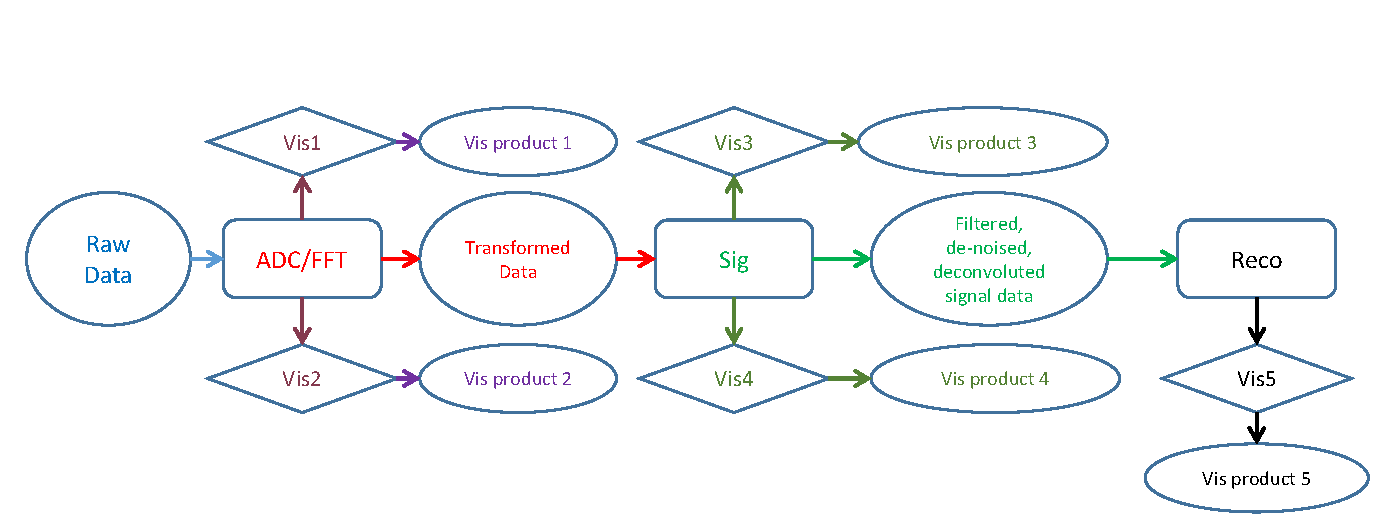
\includegraphics[width=1.0\textwidth]{figures/prompt_dag_2.pdf}
  \caption{An example of DAG representing prompt processing in \expname.}
  \label{fig:dag1}
\end{figure}
In this diagram, oval shapes represent data, rectangular blocks correspond to
elements of workload responsible for processing the data and diamonds stand for processes
which create``visual products'' (see \ref{sec:outline} and \ref{sec:viz_intro}).
The \textbf{ADC} and \textbf{FFT} components are conflated here for the following reason - while being functionally
different, both depend on data being decompressed. Since it makes sense to do decompression only once, it may
be optimal to combine these two steps in a single unit of execution.


%%%%%%%%%%%%%%%%%%%%%%%%%%%%%%%%%%%%%%%%%%%%%%%%%%%%%
\section{Design Parameters}
\label{sec:parameters}
\subsection{Staging Data for Prompt Processing}
CERN EOS appears to be the best suited platform from which to
serve the data for prompt processing for the following reasons:
\begin{itemize}

\item The online buffer is likely to operate at a significant data rate (see above) and additional I/O load on the buffer is undesirable
due to practical limits on the storage bandwidth and in order to guarantee stability of operation for the online buffer and DAQ in general.

\item It can be be expected that the data arrives to EOS rather quickly after having been captured in the online buffer (e.g.$\sim$1\,min) so
the latency due to this transfer is acceptable.

\item EOS has variety of interfaces including \xrd \cite{xrootd} which simplifies access from various types of
systems and  locations (both inside and outside the CERN perimeter).
Leveraging this capability of EOS will allow to avoid implementaion of a special data transmission handling
chain for prompt processing (such as explicit file copy to the Worker Node and back).


\end{itemize}

\subsection{Prioritization of Processing Steps}
\label{sec:priority}
Quick turnaround is the key for the prompt processing to be useful. For each processing category
to be complete it must include the visualization component in order to make the results available
to the experts. What fraction of the total stream of events ends up being processed is relatvely less
important compared to timely completion of all steps (NB. with downsampling of the data, see 
\ref{sec:downsampling}).

A use case may help to illustrate this. Let's assume a predetermined fraction of the events needs to
be reconstructed (perhaps with simplified algorithm aimed at identifying cosmic muon candidates).
This information needs to be made available to the operators as quickly as possbile in order to ascertain the performance
of the detector at a level of confidence much higher than that provided by ADC histograms.
Consider the case where the \textbf{FFT} and \textbf{Sig} parts (see \ref{sec:categories})
completed satisfactorily but are consuming a fraction of the computing resource so large that
the  \textbf{Reco} stage is starved of resources and takes a very long time to complete, making
it less relevant and less useful. This situation can be prevented by prioritizing each step higher
than the preceding one (again, with downsampling as per \ref{sec:downsampling}). In many
cases having a ``visual product'' to present the data to the operator is crucial (e.g. histograms,
event displays etc) so corresponding processes need to have sufficiently high priority.

It is therefore necessary to provide a mechanism for flexible prioritization of the different
classes of jobs running in the prompt processing system.

\subsection{Timeout}
There can be various reasons why a job may take than is practical, thus consuming valuable resources
and creating a bottleneck -- from bugs in software to a type of event which is genuinly difficult to reconstruct.
These jobs need to be triaged, diagnosed and documented separately from the main workflow and perhaps
using a different computing resource. For this reason, maximum allowed execution time (effectively a timeout)
will need to be set for each processing category in prompt processing chain.


\subsection{Workflow: Automation And State}

Prompt processing represents a use case quite different from managed production or user analysis, and is 
in essence procesing data in streaming mode. It is rather obvious that in this situation manual job submission won't scale to the
needs of the experiment, and it will be necessary to automate the prompt processing workflow.

Automation can be achieved in  number of different ways. In the simples case, processes belonging to a particular stage
of processing can be waiting for files produced by the previous stage and matching a particular name pattern
(in a fashion similar to the ``dropbox'' mechanism). This design eschews the use of a database and it is effectively
the file system which keeps the state of the workflow. For example, jobs performing calculations in the \textbf{Sig}
stage could be waiting for files containing the output of the \textbf{FFT} stage. These scheme is conceptually simple but has a number of
disadvantages, such as
\begin{itemize}
\item Matching multiple jobs to multiple files is not trivial and there may be race conditions etc
\item Detection of error status would require additional scripting
\item Likewise, generating a view of workload distribution across the processing stages is possible but requires
scripting
\item Changing characteristics of the workload is complicated
\item Bookkeeping is difficult
\end{itemize}

\noindent Problems such as listed above can be alleviated if the state of the workflow is kept in a database.
An additional and obvious advantage of this approach is that an efficient and responsive Web interface to
the system can be created with minimal effort.

\subsection{Computing Resources}
The following computing resources are being considered for prompt processing:
\begin{itemize}

\item The ``neut'' cluster  \cite{neut} at CERN (HTCondor)

\item The lxbatch facility \cite{lxbatch} at CERN (LSF)

\item Potentially, resources at a few US institutions such as FNAL and BNL.  This option is facilitated by utilizing EOS interfaces such as XRootD.

\end{itemize}

\noindent Optimally, these resources will be managed transparently in one unified system and the workload
distribution will be dynamically adjustable.

\subsection{Monitoring, Interfaces and Integration}
The requirements for the prompt processing monitoring are listed in \cite{docdb1811}.
The issues of the design of the corresponding web service and integration with other monitoring
components (such as those in DAQ) will be addressed at a later time.

The prompt processing system will need to interface with the data handling system (i.e.~F-FTS). A simple example
would be prevention of the data being purged from EOS while it's still needed for processing.

\section{The Proposed Design}
\label{sec:design}
\subsection{Summary of the Assumptions}
Most important of the design parameters itemized in Sec.\ref{sec:parameters} are

\begin{itemize}

\item An assumption that a dedicated data transfer system won't be needed for the
operation of prompt processing since the data will be read from and written to CERN EOS.

\item The workflow and its elements can be modeled as a DAG (Sec.\ref{sec:dag}).

\item Payloads within the prompt processing workflow will need to be prioritized to ensure
the quickest turnaround time possible given the resources available.

\item Timeouts will be enforced in each processing stage to ensure reliable throughput. Jobs
failing due to the timeout conditions will be logged and triaged separately.

\item A database will be used to marshal data to jobs, to keep and account for the states
of jobs in various stages of processing (including errors and failures),
and to monitor the progress of execution.

\end{itemize}

\subsection{Just-in-Time Submission}
\label{sec:justintime}
Latencies inherent in any batch system make it problematic to use common batch submission directly
since quick turnaround and throughput are required. A well known method to counter this is the use
of pilot jobs, submitted in advance and securing batch slots while optionally validating the software
environment present on the Worker Node, network connectivity and other components. The
payloads can be then distributed to primed and validated WNs immediately as the input data becomes
available, based on the desired prioritization of jobs. Alternatively, instead of running pilots it is possible to
seed the available compute element with a few classes of jobs according to \ref{sec:categories} and
let them wait till the relevant input arrives, or they time out -- this will help guarantee that
CPU cycles are not wasted by idling jobs (same actually applies to pilots). Either way, the key
here is \textit{``preemptive''} submission of pilots or jobs such that the latency of the start of job
execution is minimal. The pilot vs job decision will be made at a later time. Let us note for now that
the pilot method offers considerably more flexibility in adding additional types of jobs (payloads)
to the processing chain and modifying the distribution of resources across these different types.

\subsection{Job Queues}
The number of jobs assigned to each category listed in \ref{sec:categories} will be optimized based
on the eventual design of the processing software. For now the working assumption is that it will
be configurable so the exact number does not need to be set at this time.

Each job is characterized as its type (category), state, and references to its input and output data
(e.g.file paths for input and output). Jobs belonging to different categories are chained (see \ref{sec:categories} and \ref{sec:dag}). This is
visualized in the digram presented in Fig.\ref{fig:queues1}, which depicts three queues each containing
jobs of a specific type.

\begin{figure}[tbh]
  \centering
  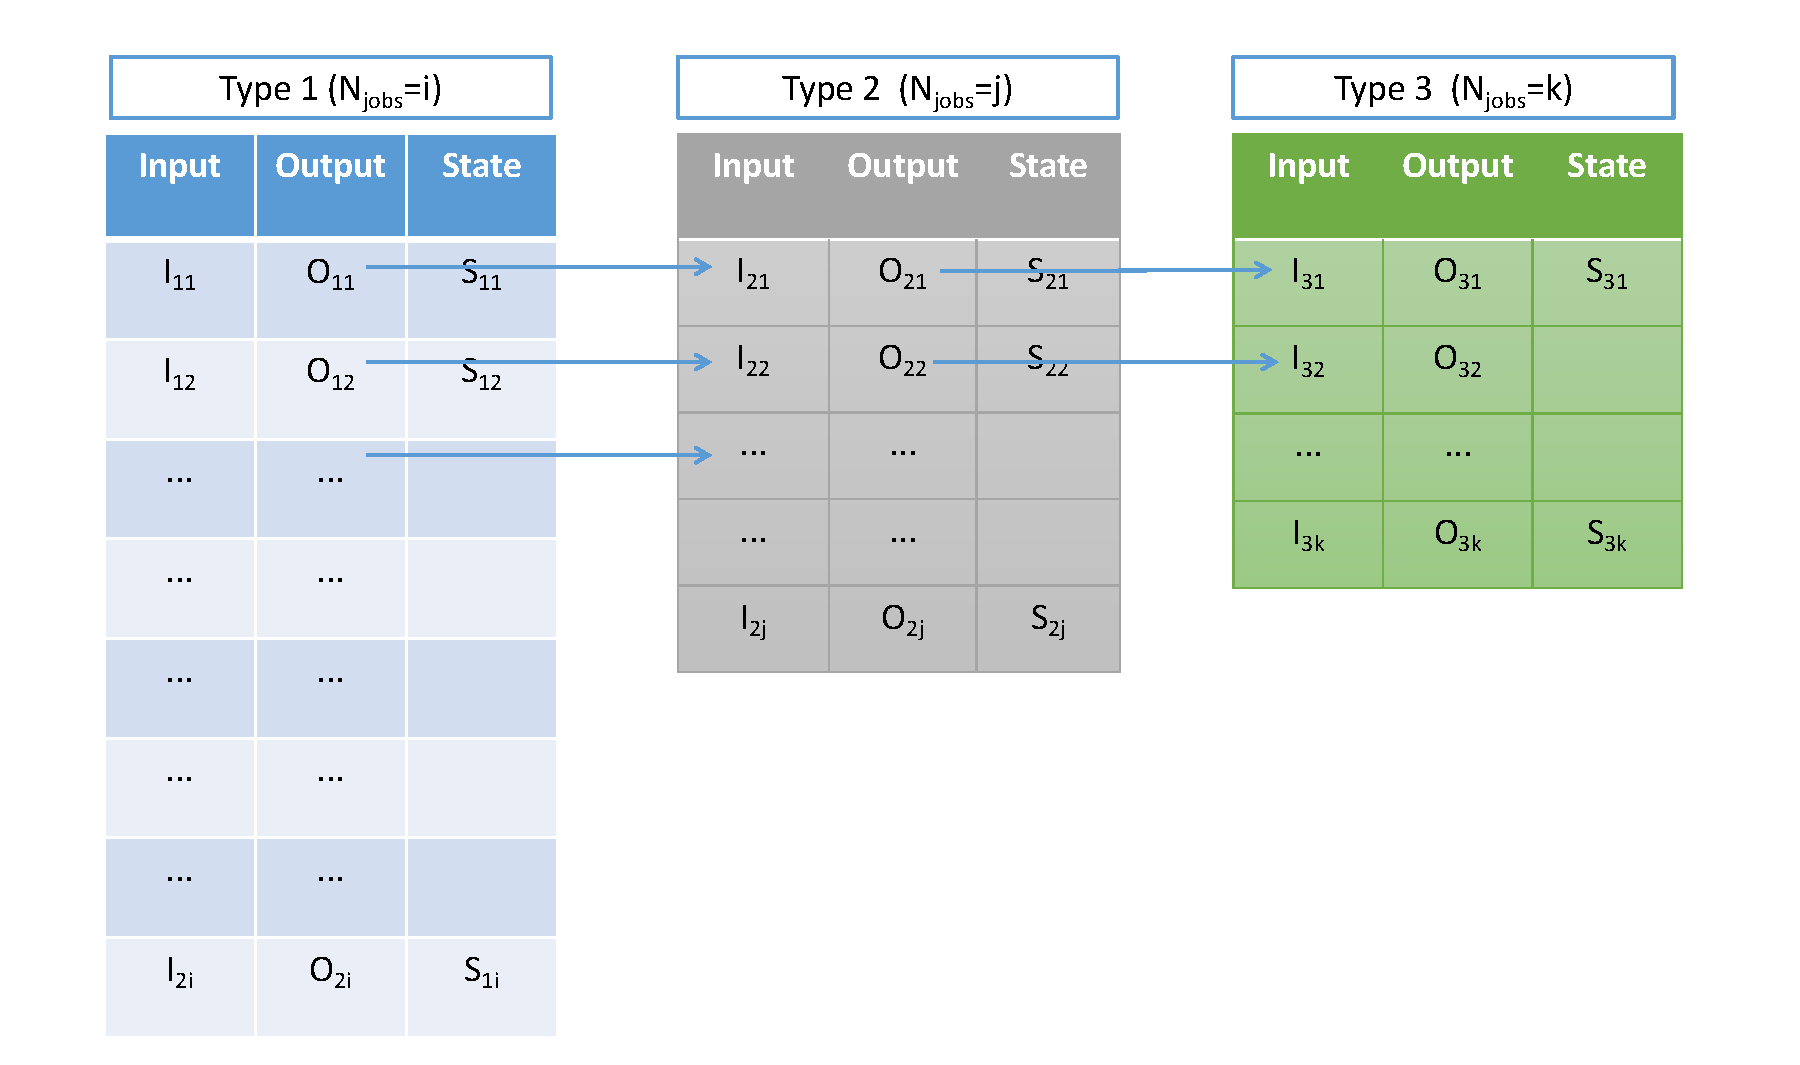
\includegraphics[width=1.1\textwidth]{figures/prompt_queues_1.pdf}
  \caption{Categories of prompt processing jobs grouped in queues. In this example, the depths of queues are different for different job types.}
  \label{fig:queues1}
\end{figure}

For example, if we consider the DAG depicted in Fig.\ref{fig:dag1}, then ``Type 1''
is \textbf{ADC/FFT}, ``Type 2'' is \textbf{Sig}, and ``Type 3'' is \textbf{Reco}. For illustration purposes,
the queues in this diagram have different depths $(i,j,k)$  -- which may indeed happen in practice.

Jobs consume data produced in the previous stage of prompt processing. For that reason, they
will need to be defined dynamically once a new pirce of input becomes available. For example,
the attribute $I_{21}$ will be assigned the value of $O_{11}$ once the corresponding $Job_1$ of Type 1
is complete. Generation of job definition is a crucial part of overall automation of prompt processing.

Keeping fixed numbers of jobs of each type running in the system at all times (with timeouts of necessary)
is indeed one design option but it may not be optimal since execution times of any job will fluctuate and there
will likely be idle jobs in some stages waiting for input.

As an alternative, the queues depicted in Fig.\ref{fig:queues1} can be conflated into a single queue
with priorities assigned to each job along the lines explained in \ref{sec:priority}. This is shown in
Fig.\ref{fig:queues2}.
\begin{figure}[tbh]
  \centering
  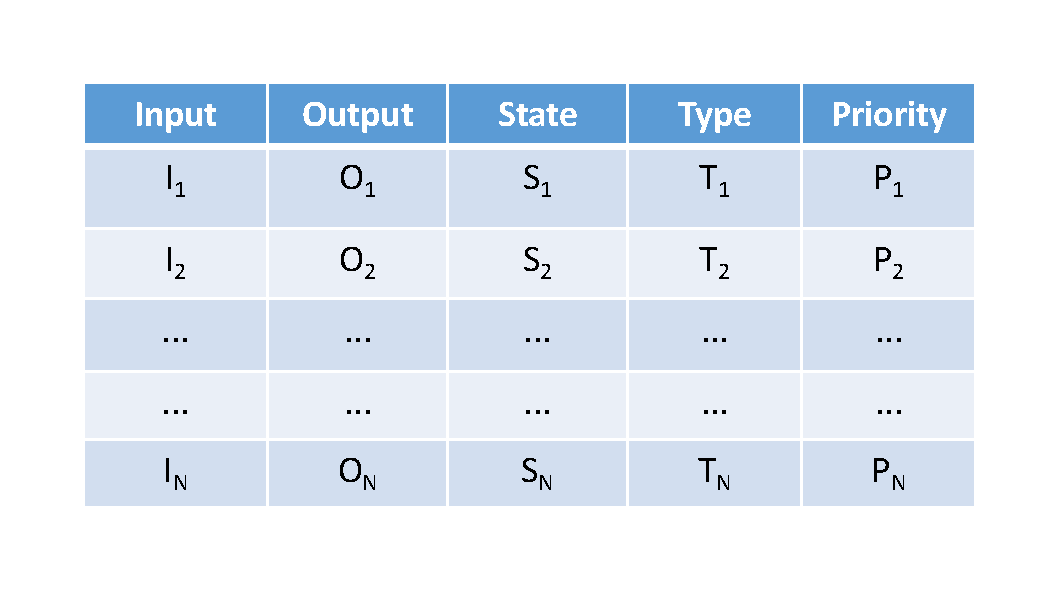
\includegraphics[width=0.85\textwidth]{figures/prompt_queues_2.pdf}
  \caption{The unified queue of prompt processing jobs.}
  \label{fig:queues2}
\end{figure}
Jobs now have additional attributes, such as the type and priority.
The depth of such queue will be set according to the available number of Worker Nodes assigned for
prompt processing (e.g. it can be a certain portion of the ``neut'' cluster and a certain number of batch slots on
lxbatch). There are several ways to ensure that higher priority jobs are placed in the queue (for example by
dropping jobs of lower priority still in the ``wait'' condition) and the exact method will be chosen at a later time.

Let us assume that the pilot method is chosen for ``just-in-time'' job submission (see \ref{sec:justintime}). In this
case, the following is a possbile scenario of how this unified queue will operate, assuming it is implemented
as a database table:
\begin{itemize}

\item A fixed number of pilot jobs (wrapper scripts) are submitted to the available batch facilities (which can include both
lxbatch and ``neut'' but potentially also other sites such as FNAL).

\item Because of possible timeouts, completions and error conditions encountered by the pilots their number will naturally
diminish over time so it must be replenished in order to remain at an appropriate level. This can be achieved by reusing
existing software created for this purpose in other experiments (e.g. the AutoPyFactory from ATLAS).

\item Data arriving from DAQ and its online buffer to EOS triggers the mechanism which makes entries in the queue for the
first stage of processing (e.g. ADC/FFT). Entries for this first stage are arraned in the LIFO manner. In other words, preference
in the queue order is given to the most recent data detected, in order to ensure that the output contains the freshest
data to help the processing remain prompt and current. Note that this is different from conventional production or analysis --
first of all, processing is done on a fraction of data, and second, the data is prioritized by its timestamp.

\item A broker process is listening to HTTP messages from the pilots signaling that they are ready to accept their payload.

\item A table sweep selects the job entries of the highest priority and replies to the pilot's HTTP request with information
sufficient for locating and initiating the correct payload (this can be a URL point to a script etc).

\item Upon the payload assignment, the pilot notifies the broker about its status and the state of the job (e.g.
that the execution started, or some kind of error was encountered).

\item The job record is then updated based on this information. For example, the state of the job can undergo the following
transitions  during the process described above: from ``waiting'' state to ``being assigned'' state to ``running'' state.

\item Upon completion, the pilot send notification to the broker, the queue is updated with the state information (the job is ``finished'') and
a new entry is made in the queue for the next stage of processing, with input defined as the data coming from the stage that just completed.

\item This process is iterative by nature, i.e.~the following stages operate in the same manner as links in the processing chain.

\item The ``visual products'' created throughout the processing chain are exported to a Web service to create the presentation
layer for the end user.

\item Parts of the output from all stages which are deemed to be of value for record keeping and for additional
diagnostics are committed to long term storage (possibly utilizing F-FTS and SAM). This functionality can be included
in the general cleanup logic -- most of the data in the chain won't need to be persisted and can be deleted once
execution of the corresponding DAG completes, while a few data elements will be sent to storage. This can be
implemented as a periodic table sweep and application of rules which will be configurable.

\end{itemize}

\section{Summary}
A design of the Prompt Processing system for \expname is proposed. Variations are possible
while the version which currently appears optimal is outlined below:


\begin{enumerate}

\item The pilot job mechanism is proposed to minimize latencies inherent in the Grid and general batch system job submission.
A pilot can be thought of as a payload-agnostic wrapper script which includes the functionality necessary to communicate
with the Web service distributing payloads and keeping the state of the workflow.

\item Arrival of raw data from DAQ triggers generation of entries in the job queue implemented as a database table.

\item Different payloads which are parts of the Prompt Processing system will be assigned different priorities in order to ensure
adequate throughput and timely delivery of the results to the end user. The priorities may be dynamically changing based on
the state of the set of DAGs currently being processed. For example, more resources may be allocated to longer DAGs which already
completed a few stages, in order to reach results more quickly. There may be a few ``hot slots'' left idling to be able to quickly
start execution of the highest priority jobs (such as the final reconstruction stage). The exact mechanism will be determined
at a later time.

\item Payloads are matched to pilots according to priorities.

\item The pilots initiate the execution on the WNs where they run.

\item The state of each job is updated in the database based on messages received from the pilot.

\item The database also serves as the basis for the monitoring monitoring and debugging.

\item Completion of each job results in adding another entry to the queue with priority set according to the processing stage as
explained in \ref{sec:priority} (unless this is a leaf in the DAG describing the workflow).

\item Visual products and other data required by the operators of the experiment are made available via a Web service.
A predetermined fraction of the data produced by various stages of the prompt processing is committed to long storage
for record keeping.


\end{enumerate}

\clearpage
\begin{thebibliography}{1}
\bibitem{docdb1086}
{DUNE DocDB 1086: \textit{ protoDUNE/SP data scenarios with full stream (spreadsheet)}}\\
\url{http://docs.dunescience.org:8080/cgi-bin/ShowDocument?docid=1086}

%\bibitem{docdb186}
%{DUNE DocDB 186: \textit{ ProtoDUNE Proposal}}\\
%\url{http://docs.dunescience.org:8080/cgi-bin/ShowDocument?docid=186}


%\bibitem{docdb1209}
%{DUNE DocDB 1209: \textit{Basic Requirements for the protoDUNE Raw Data Mangement System}}\\
%\url{http://docs.dunescience.org:8080/cgi-bin/ShowDocument?docid=1209}


\bibitem{docdb1212}
{DUNE DocDB 1212: \textit{Design of the Data Management System for the protoDUNE Experiment}}\\
\url{http://docs.dunescience.org:8080/cgi-bin/ShowDocument?docid=1212}

\bibitem{docdb1811}
{DUNE DocDB 1811: \textit{Prompt Processing System Requirements for the Single-Phase protoDUNE}}\\
\url{http://docs.dunescience.org:8080/cgi-bin/ShowDocument?docid=1811}


\bibitem{xrootd}
{XRootD}\\
\url{http://www.xrootd.org}

\bibitem{neut}
{Neutrino Computing Cluster at CERN}\\
\url{https://twiki.cern.ch/twiki/bin/view/CENF/NeutrinoClusterCERN}

\bibitem{lxbatch}
{The CERN batch computing service}\\
\url{http://information-technology.web.cern.ch/services/batch}

\end{thebibliography}


\end{document}